\subsubsection{Modelo Eventos/Transacciones}

El modelo eventos representa una transacción base a todos los componentes que posteriormente modelaremos.

%A continuación podemos ver en la figura \ref{fig:modelo_events_ecore} como es representado este modelo. Consiste en dos modelos: \textit{Event} (Evento) , y \textit{Actuator} (Actuador). 

%\begin{figure}[htp]
%	\centering
%    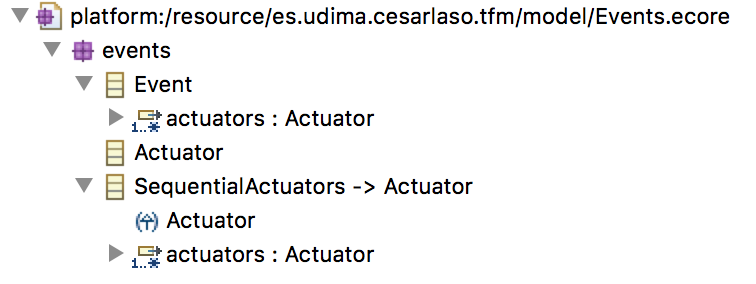
\includegraphics[height=0.3\textheight]{images/emf_capturas/events_ecore.png}
%    \caption{Modelo Events. Visualización formato ecore}
%    \label{fig:modelo_events_ecore}
%\end{figure}



\paragraph{Modelo evento}.
El modelo \textit{Evento} representa una entidad la cual es capaz de generar por sí misma acciones, permite definir los eventos del sistema. Estos pueden ser de diferente naturaleza: aperiódico y periódico.

Como ejemplo de evento aperiódico contamos con un evento de entrada/salida, como puede ser un cambio de estado en una entrada digital. Como ejemplo de evento periódico, contamos con un temporizador el cual es ejecutado cada x unidades de tiempo. 

Un evento siempre contendrá uno o varios actuadores. Un evento sin actuadores no tiene sentido con lo que no está permitido en el modelo.



\paragraph{Modelo actuador}.
El modelo actuador representa una acción a realizar por parte del sistema. Los actuadores dentro del evento se lanzarán de forma concurrente todos al mismo tiempo sin esperar a la finalización de cada uno de ellos. Si fuera necesario mantener un orden en los actuadores, es necesario utilizar el modelo contenedor \textit{SequentialActuactor} el cual en su funcionamiento ejecuta el grupo de actuadores secuencialmente uno tras otro, esperando a la finalización de un actuador para invocar al siguiente.

A continuación en la figura \ref{fig:modelo_events_classes} podemos visualizar esta representación mediante un diagrama de clases.

\begin{figure}[htp]
	\centering
    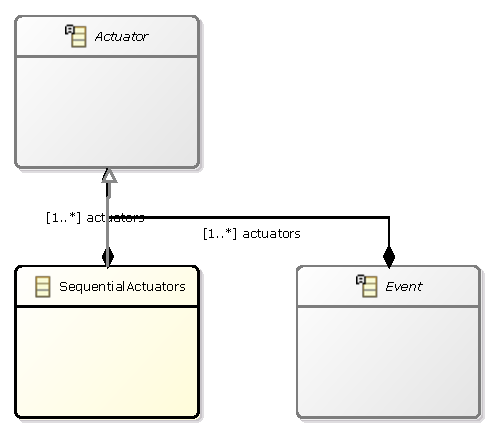
\includegraphics[height=0.3\textheight]{images/models/events_class_diagram.pdf}
    \captionmodeloclase{Eventos / Transacciones}
    \label{fig:modelo_events_classes}
\end{figure}

%\clearpage
